\documentclass[english,12pt,twoside,a4paper]{report}
\usepackage[T1]{fontenc}
\usepackage[english]{babel}

% Use References instead of Bibliography
\addto\captionsenglish{\renewcommand{\bibname}{References}}

% for harvard style referencing
\usepackage{natbib}

\usepackage{appendix}

% Start table formatting
\usepackage{array,etoolbox} 
% End table formatting

%\usepackage{minted}
\usepackage{minted}
\setminted[python]{breaklines}

% Times new roman
%\usepackage{mathptmx} % Times new roman
% graphics 
\usepackage{graphicx}
\graphicspath{{images/}}

% for adding hyper linking
\usepackage[%
	colorlinks=true,
	pdfborder={0 0 0},
	linkcolor=red
]{hyperref}

% cleverreferecing 
\usepackage[nameinlink,noabbrev]{cleveref}
% geometry to manage page size and more 
\usepackage[a4paper,width=150mm,top=20mm,bottom=20mm,bindingoffset=6mm]{geometry}

% footer and header
\usepackage{fancyhdr}
% \pagestyle{fancy}

% customize header
\fancyhead{} % clear header

% customize footer
\fancyfoot{} % clear footer
\fancyfoot[C]{\thepage}

% align images package start
\usepackage{caption}
\usepackage{subcaption}
% align images package end
\renewcommand{\thechapter}{\ifcase\value{chapter}\or ONE\or TWO\or THREE \or FOUR\or FIVE\else Many\fi}
\renewcommand{\chaptername}{\MakeUppercase{CHAPTER}\centering{}} % changes Chapter One to CHAPTER ONE


\begin{document}
	% input the title page 
	\pagestyle{empty}
		\begin{titlepage}
	\begin{center}
		\line(1,0){300}\\
		[0.25in]
		\huge{\bfseries Data Mining and Informatics}\\
		[2mm]
		\line(1,0){200}\\
		[1.0cm]
		By \\
		[1.0cm]
		\textsc{\LARGE \bfseries Ifeanyi Nnamdi Okoli}\\
		\textsc{\LARGE \bfseries 2348748}\\
		[2cm]
		\bfseries Department of Computer Science with Artificial Intelligence\\
		In partial fulfillment for the award of Master's Degree (M.Sc.) in Computer Science \\
		[1in]
		March 12, 2025\\
		[2mm]

	\end{center}
\end{titlepage}
	
	\pagenumbering{roman}
	\tableofcontents
	
%\chapter*{Declaration}

%\addcontentsline{toc}{chapter}{Declaration}
	
%\input{preliminaries/dedication}
%\addcontentsline{toc}{chapter}{Dedication}
	
%\chapter*{Acknowledgment}
%\addcontentsline{toc}{chapter}{Acknowledgement}
	
%\input{preliminaries/listoffigures}
%\addcontentsline{toc}{chapter}{List Of Figures}
	
%\preto\tabular{\setcounter{magicrownumbers}{0}}
%\newcounter{magicrownumbers}
%\newcommand\rownumber{\stepcounter{magicrownumbers}\arabic{magicrownumbers}}
%\section{List of Tables}

	
%	\begin{tabular}{@{\makebox[1em][r]{\rownumber\space}} | l@{\makebox[1em][r]{}} | l}
%		
%		\multicolumn{0}{@{\makebox[01em]{ID~}} | } | { Features jsdfjsfj sdfj ds df dlfsd fd} | { Featurezz}\\    
%		Something & hello\\
%		Other stuff & hello \\
%		Something something & hello \\
%		MAGIC!  & hello\\ 
%		Something something & hello
%	\end{tabular}
\tableofcontents
%\addcontentsline{toc}{chapter}{List Of Tables}
	
%\addcontentsline{toc}{chapter}{Appendix}

	\clearpage
	
	\pagestyle{fancy}
	\chapter{Project Tools Used}
	\pagestyle{fancy}
The project just like any other project require some certain tools for its proper execution. Having carefully examined the tasks ahead, some certain tools of the trade were chosen. Below is a few of the chosen tools (or technologies) and their description. 
\begin{enumerate}
	\item \textbf{Data Manipulation Tools}
		\begin{enumerate}
			\item Numpy - The full meaning of numpy is numerical python. As such, it is a python package used for numerical computation and manipulation of data. Numpy is free and open source, hence one can use it as wished and can also contribute to it code base, is it is maintained by the open source community. For more, check out the documentation \cite{NumPyDocumentation}
			
			\item Pandas - Pandas, a table or spreadsheet-like data manipulation tool or framework is used to handle and crunch. Pandas effectively handles excel, csv, tsv and others. Pandas looks much like excel but much more than excel. \cite{PandasDocumentationPandas}
		\end{enumerate} 
	\item \textbf{Visualization Tools}
		\begin{enumerate}
			\item Matplotlib - Matplotlib is a visualization library commonly used in python data analytics. It is very easy to learn and use and it is very new-user friendly, being considered the most common very first visualization library for python users. To see the documentation and tutorial on what pandas is and what it is used for, [see][]\cite{GettingStartedPandas}
			\item Seaborn - Seaborn is a more sophisticated and advanced visualization library using python. Seaborn was written on top of the matplotlib library. See \cite{IntroductionSeabornSeaborn}
		\end{enumerate} 
		
	\item \textbf{Algorithm and Methodology}Givenn that the outcome that will be predicted is a categorical data, the algorithm methodology to be employed is going to be classification algorithm. This implies that the data set would be label encoded to transform categorical features to numeric features, standardized to ensure that all the data points are in the same scale.


\end{enumerate}

	\pagenumbering{arabic}
	\setcounter{page}{1}
	
	\chapter{Dataset}
	\pagestyle{fancy}
\section{Data Collection \& Understanding}%\label{sec:background}
The dataset, titled \bfseries{Student Performance \& Behaviour Dataset} is a dataset of 5000 records collected from a private learning provider. It contains 5000 records and 23 features.  \cite{StudentPerformanceBehavior} of different and diverse students' behaviors and environmental factors that go a long way, directly and or indirectly affecting a students academic performance. And it has key student attributes necessary for exploring patterns, correlations and insights related to academic performance. Below is the data dictionary table 

\begin{enumerate}
	\item \textbf{Data Dictionary}
	\begin{enumerate}
		\item Student\_ID: Unique identifier for each student
		\item First\_Name: Student's first name 
		\item Last\_Name: Student's last name 
		\item Email: Contact email (can be anonymized)
		\item Gender: Male, Female and Other
		\item Age: The age of the student
		\item Department: Student's department (e.g., CS, Engineering, Business).
		\item Attendance (\%): Attendance percentage (0-100%).
		\item Midterm\_Score: Midterm exam score (out of 100).
		\item Final\_Score: Final exam score (out of 100).
		\item Assignments\_Avg: Average score of all assignments (out of 100).
		\item Quizzes\_Avg: Average quiz scores (out of 100).
		\item Participation\_Score: Score based on class participation (0-10).
		\item Projects\_Score: Project evaluation score (out of 100).
		\item Total\_Score: Weighted sum of all grades.
		\item Grade: Letter grade (A, B, C, D, F).
		\item Study\_Hours\_per\_Week: Average study hours per week.
		\item Extracurricular\_Activities: Whether the student participates in extracurriculars (Yes/No).
		\item Internet\_Access\_at\_Home: Does the student have access to the internet at home? (Yes/No).
		\item Parent\_Education\_Level: Highest education level of parents (None, High School, Bachelor's, Master's, PhD).
		\item Family\_Income\_Level: Low, Medium, High.
		\item Stress\_Level (1-10): Self-reported stress level (1: Low, 10: High).
		\item Sleep\_Hours\_per\_Night: Average hours of sleep per night.
		
	\end{enumerate} 	
\end{enumerate}



%\subsection{Medicinal Properties}
%\subsection{Preservation methods}
%\subsection{Phytochemical content of Ugu}

%\section{Problem Statement}
%\section{Objective of the Study}
%\section{Research Questions}
%\section{Justification of the study} % (Significance of the study)}
%\section{Scope of the Study}
	
	\chapter{Data Preprocessing}
	In this project, the very first task was to import the libraries that will be used in this project. I prefer to import all my libraries at the beginning and this enables me to debug faster given that I have a single library import cell.
Below is the code snippet\\
\section{Import Libraries}
	\bf import libraries needed for the task
\begin{minted}
	{python}
	# import needed libraries
	import numpy as np
	import pandas as pd
	import matplotlib.pyplot as plt
	import seaborn as sns 
	from IPython.display import Markdown as mkd 
\end{minted}
After libraries importation (which is iterative until the project is completed)  the next step in data analytics is to import and pre process the data. Data pre-processing is a collection of investigative actions performed on data prior to the actual analysis being performed. 
The first step is to import the dataset into the working environment, mostly but not limited to jupyter notebook. This was done with the python code snippet
\newpage
\section{Data Preprocessing}
\bf load the dataset
\begin{minted}{python}
	# load the dataset in the df variable
	df = pd.read_csv("datasets/Students_Grading_Dataset.csv")
	
	# convert all features to lovercase 
	df.columns = [col.lower() for col in df.columns]
\end{minted}

\section{Data Shape} 
Data shape is a term used too describe how many rows and columns are in the dataset. Here, I used markdown imported as `mkd` to print out a statement that shows we have 5000 rows (entries) and 23 columns, features or attributes of each entity in the dataset.See Figure \ref{fig:data_shape}

\section{Data Head and Tail}
Data head an tail, were respectively used to glimpse at the first and last five entries of the dataset. We these, we got our first knowledge of the content of the dataset from the top and the bottom.
See data head Figure \ref{fig:data_head} and see data tail Figure \ref{fig:data_tail}

\section{Null Values}
Data, being sourced from many possible sources is mainly always noisy containing both empty values, unwanted and unexpected values introduced by both human errors in the case of human data entry and system glitches when the data are sourced from sensors and other automated devices. For this reason, I checked to see if there was any null value or invalid entry. Total number of null values Figure~\ref{fig:total_null_values} and duplicates.  Null values distribution Figure~\ref{fig:null_values_dist}

\section{Basic Descriptive Statistics}
This is what I use to first check if there is an outlier in the dataset. This works only for numeric feature and does not work for categorical features. Here is the the formulat 1.5 * IQR. Any number outside of this range, in both positive and negative directions (+ or -  signed) is considered an outlier. This is followed by a boxplot to confirm the outlier or disprove it. This is as shown in igure~\ref{fig:desc_stat}

\section{Inconsistent Grading System}
From the results below, grading inconsistency is discovered A 78.89 final\_score and 66.13 total\_score were graded F on line 5 while on line 4997, a 644.21 final\_score and 54.25 total\_score were graded as A. No attem is made yet to investigate why it existed given the task at hand and time. A fix is provided, using a function to calculate grades based on final\_score and created a new feature called grade\_corrected. Inconsistent grading Figure~\ref{fig:inconsistent_grades}

\begin{minted}{python}
	# These are the functions used in the task
	
	# function to fix grading inconsistent issue.
	"""
	Using; https://www.mastersportal.com/articles/2290/how-to-convert-uk-grades-for-masters-degrees-in-other-countries.html
	
	Converting British grades into American grades
	In the US, the grading system uses letters A-F (without E) to evaluate students. D is the minimum passing grade.
	
	+70% = A
	60-69% = B
	50-59% = C
	40-49% = D
	Below 40% = F (fail)
	"""
	def grader(total_score):
	"""
	This function is used to compute grades for the students. 
	This also applies a known, global and generally accepted grading system.
	The input is the total score.
	"""
	"""Grades : A, B, C, D, E, F"""
	if isinstance(total_score, int) or isinstance(total_score, float):
	if total_score < 40:
	return 'F'
	# elif total_score <= 50:
	#     return 'E' 
	elif total_score <= 49:
	return 'D' 
	elif total_score <= 59:
	return 'C'
	elif total_score <= 69:
	return 'B' 
	else:
	return 'A'
	else:
	raise "Wrong value type. Int or float required" 
	
	
	
	# apply the the to create the grade_corrected feature
	stud_record['grade_corrected'] = stud_record['total_score'].apply(grader)
	
	
	# show grading inconsistency once more, 
	# investigate accurate fix
	stud_record[['final_score', 'total_score', 'grade', 'grade_corrected']].head()
\end{minted}

The Figure \ref{fig:sample_grade_corrected} is the sample of the grade\_corrected feature just created
	
	\chapter{Exploratory Data Analysis (EDA)}
	Exploratory Data Analysis, EDA is the exploration of the data to discover patterns and trends prior to training a model. 

\section{Univariate Data Analysis}. Univariate analysis is the simplest form of analyzing data. “Uni” means “one”, so in other words, your data has just one variable. It does not deal with causes or relationshiops (unlike what regression analysis does) and its major purpose is to describe, it takes data and summarizes that data and finds trends and patterns in them.

\subsection{Gender Distribution}
Checking the dataset, running the code to check for number of each gender
\begin{minted}{python}
# students gender distribution
gender_distr = stud_record.groupby(by='gender').size()

gender_distr.plot(kind='bar')
plt.title('Student Gender Distribution', fontdict={'size':14, 'fontweight':'bold'})
plt.xlabel('Student Gender', fontdict={'fontweight':'bold'})
plt.ylabel('Gender Count', fontdict={'fontweight':'bold'})
plt.ylim(2400, 2600)
plt.grid()

# show gender distribution figures
gender_distr
\end{minted}
This generated figure ~\ref{fig:gender_dist}


\subsection{Student Age Distribution}
Here student age distribution was investigate. This was done to ascertain that the student population is of the expected student age and not of elderly people or underaged. From the result got, it is proved that the student are of student ages ranging from 18 years old to 24 years old. It is also observed that the ages are closely distributed within the range of 682 for 18 years of age (the minimum) to  24 years old (the maximum age), the highest age.
The investigation code is as shown below: 
\begin{minted}{python}
# student age distribution
age_dist = stud_record.groupby(by = 'age').size()
age_dist.plot(kind='bar')
plt.ylim(600, 800)
plt.grid()
plt.title("Student Age Distribution", fontdict={'size':14, 'fontweight':'bold'})
plt.xlabel('Student Age', fontdict={'fontweight':'bold'})
plt.ylabel("Student Age Count", fontdict={'fontweight':'bold'})


# pd.DataFrame([age_dist.values, age_dist.index], columns=['Numbers', 'values'])
age_dist.index
pd.DataFrame({'Age Group': age_dist.index, 'Age Group Count': age_dist.values})
\end{minted}
As pictorized in Figure \ref{fig:stud_age_dist}


\subsection{Department Distribution}
Let find out what departments / fields of study that are represented in our student population. Not just what departments or fields that are represented but also to find what population of our students are in these departments. 
The code snippet below was used for the investigation
\begin{minted}{python}
# group dataset by department and get size of each department
dept_dist = stud_record.groupby(by='department').size()
dept_dist.plot(kind='bar')
plt.title('Department Distribution', fontdict={'size':14, 'fontweight':'bold'})
plt.xlabel('Department', fontdict={'fontweight':'bold'})
plt.ylabel('Department Count', fontdict={'fontweight':'bold'})
plt.grid()
# plt.show()

pd.DataFrame({'Department':dept_dist.index, "No. of Students": dept_dist.values})
\end{minted}

In figure, Figure \ref{fig:dept_dist} shows the department and number of students in them. 


\subsection{Attendance Distribution [First 100]}
The rate of attendance of students, in an attempt to identify what could be related to student performance / grade. 
The code below was used. As can be seen in the chart, the output is much like a timeseries result. Given that this is outside the scope of this task, further investigation was not carried. 

\begin{minted}{python3}
# plot student attendance
stud_record['attendance (%)'].plot()
plt.title("Attendance Plot [First 100]", fontdict={'size':14, 'fontweight':'bold'})
plt.xlabel("Student Attendance", fontdict={'fontweight':'bold'})
plt.ylabel("Student Attendance (%)", fontdict={'fontweight':'bold'})
plt.xlim(1, 100)
plt.show()
\end{minted}
Assignment avg, Quizzes avg and study hour per week shared the same pattern and the same thing could be said about them. Moving on

\subsection{Internet Home Acess Distribution}
The internet has had a profound and far-reaching effect on students' studies, revolutionising the way they access
information, interact with educational content, and collaborate with others. \cite{article}. The use of internet, in short while has affected all aspects of human with human education at the center of it all. Hence, the search to see patterns how internet access at home could affect or influence student performance. 
The code snippet is as below: 
\begin{minted}{python}
# dataset grouping by internet_access_at_home and getting the sizes
internet_access_at_home = stud_record.groupby(by='internet_access_at_home').size()

internet_access_at_home.plot(kind='bar')
plt.title('Student Internet Home Access Distribution', fontdict={'size':14, 'fontweight':'bold'})
plt.xlabel('Home Internet Accesss', fontdict={'fontweight':'bold'})
plt.ylabel('Home Internet Access Count', fontdict={'fontweight':'bold'})
# plt.ylim(2400, 2600)
plt.grid()
\end{minted}

According to Figure \ref{fig:stud_home_internet}, most of the students have internet access at home as suspected. 

\subsection{Student Family Income Level Distribution}
Let find out the income level of the parents of the students in the dataset. From Figure \ref{fig:income_level}, it is evedent that most, almost of the students are from Low to Medium Income Earners, maybe workers and not business owners. 


\subsection{Student Stress Level Distribution}
Stress, personally seen as a by-product of hardwork affects humans in all endeavour. Students are not going to be of any exception. Hence let check / investigate the student calibrated stress level from the dataset. The code snippet is : 

\begin{minted}{python}
# group dataset by stress_level(1-10) and get size of each stress level
stress_level = stud_record.groupby(by='stress_level (1-10)').size()
stress_level = pd.DataFrame(stress_level) 
stress_level.plot(kind='bar')
plt.title('Student Stress Level Distribution', fontdict={'size':14, 'fontweight':'bold'})
plt.xlabel('Student Stress Level', fontdict={'fontweight':'bold'})
plt.ylabel('Student Stress Level Count', fontdict={'fontweight':'bold'})
plt.ylim(400)
plt.grid()
plt.show();
\end{minted}

This is brought to live by Figure \ref{fig:stress_level}

\subsection{Parent Education Level}
This is yet another factor that is expected to have great effect on students academic work success rate. 
Among those salient factors are parent’s occupation, educational
attainment, socioeconomic status, family composition, parental involvement, peer and teacher influence, and adolescent self-efficacy \cite{nelson_impact_nodate}. 
I looked at the parent education level of students using the python code snippet below:
\begin{minted}{python}
# dataset grouped by paretn_education_level and the different sizes obtained
parent_education = stud_record.groupby(by='parent_education_level').size()
parent_education.plot(kind='bar')
plt.title("Parent Education Level", fontdict={'fontweight':'bold', 'fontsize':14})
plt.xlabel('Parent Education Level', fontdict = {'fontweight':'bold', 'fontsize':10})
plt.ylabel('Count', fontdict={'fontweight':'bold', 'fontsize':10})
plt.grid()

plt.show();
\end{minted}

And this generated the Figure \ref{fig:parent_edu}

\subsection{Extra Curricular Activities Dist}
It is a popular saying that all work and no play makes Johny a dull boy. Students are expected to engage in other extra curricular activites like games and sports to name just a few.
Unfortunately, it is clear that more than half of the students do not engage in extra curricular activities. This could point to something. Who knows? The snippet for the data investigation is below : 
\begin{minted}{python}
# data grouped by extra curricular activities of student. Size of yes / no extracted
extracurricular = stud_record.groupby(by='extracurricular_activities').size()

extracurricular.plot(kind='bar')
plt.title('Extrac Curricular Activities Dist', fontdict={'fontweight':'bold', 'size':14})
plt.xlabel('Extrac Curricular Activities', fontdict={'fontweight':'bold', 'size':10})
plt.ylabel('Extra Curricular Count', fontdict={'fontweight':'bold', 'size':10})
plt.grid()
plt.show()
\end{minted}
And the accompanying figure is Figure \ref{fig:extra_curricular}

\subsection{Student Grade Distribution}
Here, let see what grades are available. It is clear that students are graded by A, B, C, D and F. But from the chart, students only scored A, B, and C. No D or F. Impressive! The code snippet used is below: 
\begin{minted}{python}
# group dataset by grade_corrected and get size of each grade
grade = stud_record.groupby(by='grade_corrected').size()
grade.plot(kind='bar')
plt.title("Student Grades", fontdict={'fontweight':'bold', 'size':14})
plt.xlabel('Grades', fontdict={'fontweight':'bold', 'size':10})
plt.ylabel('Grade Count', fontdict={'fontweight':'bold', 'size':10})
plt.grid()

plt.show()
\end{minted}

The code snippet above generated the visualisation : Figure \ref{fig:stud_grade}


\section{Bivariate Data Analysis}
This is the analysis of features in association with other features and the essence is to find how features relate to each other. This helps in predictability of one feature based on another feature.
 involves looking at two variables at a time. Bivariate EDA can help you understand the relationship between two variables and identify any patterns that might exist \cite{chip_types_2023}
 
 \subsection{Gender Grade Distribution}
 Wondering if the ability if the ability to score high or low can be gender based? I assure you that you are not alone in that. Let see what our data has to say if that ability is or can be gender based. The investigation was done with the python code snippet below
 
\begin{minted}{python}
# group dataset by grade_corrected and gender
gender_grade = stud_record.groupby(by=['grade_corrected', 'gender']).count()['student_id'].reset_index()
gender_grade

valuez = np.array(gender_grade['student_id'])
rows = gender_grade['grade_corrected'].unique() # rows to be plotted
num_rows = int(len(gender_grade['grade_corrected'].unique())) # num of rows for reshaping
num_cols = int(len(gender_grade) / len(rows))   # num of cols for reshaping

data = pd.DataFrame(valuez.reshape((num_rows, num_cols)),
index=pd.Index(list(rows), name='grade'),
columns=pd.Index(['female','male'], name=''))
data = data.reset_index()
data
\end{minted} 

The gender grade distribution figure / number is as in Figure \ref{fig:gender_grade_nums} and show in bar chart in Figure \ref{fig:gender_grade_fig}
From the results got from gender grade distribution, good grades or academic success might not depend on gender. As any one, female or male has the potential to put in good work and succeed. Other things would really affect students's success rate but not their gender. The different grades, A, B and C has balanced distribution of the number of female and male who obtained such grades. 



\subsection{Grade By Department Distribution}
Now considering grade by department distribution, one could ask if it is possible that the course of study could help boost students' success. Well, we have the and just have to ask the data to have, on the least an insight. 
The python code snippet :

\begin{minted}{python}
# investigation of grade-department relationship
department_grade = stud_record.groupby(by = ['grade_corrected', 'department']).size().reset_index()
department_grade

rows = department_grade['grade_corrected'].unique() # rows to be plotted
num_rows = int(len(department_grade['grade_corrected'].unique())) # num of rows for reshaping
num_cols = int(len(department_grade) / len(rows))   # num of cols for reshaping

data = pd.DataFrame(department_grade[0].values.reshape(num_rows, num_cols), 
index=pd.Index(list(rows), name='grade'),
columns = department_grade['department'].unique()
)
data = data.reset_index()

grades = tuple(data['grade'].values)
scores = {
	data.columns[1] : tuple(data[data.columns[1]].values),
	data.columns[2] : tuple(data[data.columns[2]].values),
	data.columns[3] : tuple(data[data.columns[3]].values),
	data.columns[4] : tuple(data[data.columns[4]].values),
}

x = np.arange(len(grades))
width = 0.25 # bar width
multiplier = 0

fig, ax = plt.subplots(layout='constrained')

for attribute, measurement in scores.items():
offset = width * multiplier 
rects = ax.bar(x + offset, measurement, width, label = attribute)
ax.bar_label(rects, padding=3)
multiplier += 1

# Add some text for labels, title and custom x-axis tick labels etc
ax.set_ylabel("ylable")
ax.set_title("Title here", fontdict={'fontweight':'bold', 'size':14})
ax.set_xticks(x + width, rows)
ax.legend(loc='upper right', ncols = len(rows) - 1)
# ax.set_ylim()
plt.xlabel('Grades', fontdict={'fontweight':'bold', 'size':10})
plt.ylabel('Department Grade Distrution', fontdict={'fontweight':'bold', 'size':10})
plt.title('Department Grade Distribution', fontdict={'fontweight':'bold', 'size':14})

plt.show()
\end{minted}

is telling us that department / course of study could help student's performance. Yes I have that believe too. But then it would not depend on the course of study only as other factors would come in to play. Factors like:
\begin{itemize}
	\item Passion :  As passion is a huge factor in success rate, students studying programs they are passionate about can, affect their rate of success in those fields. This could be encouraged by the trending computing fields in the social media and everyday living.
	
	\item Resource Availability: This is how easy it is for students to access materials relating to their course of study. It could be from the physical or digital library or the internet and even from peers. 
	
	\item Social Trend : What is trending at the time. It is common knowledge that everyone at the moment is talking about Machine Learning, Data Science, AI and Deep Learning. All these fields are the children of computer. Hence their trending could make computer science, the leading department is in good grades much more interesting to study. 
\end{itemize}
According to the data, Computer Science (CS) is a leading programme in academic performance with Computer Science outperforming others in A, B or C grades with greater margin in A grade.

\subsection{Attendance Grade Distribution}
Now moving forward investigating into whether attendance to classes has positive effect on academic performance. Checking if, as is popularly said, that punctuality is the soul of business. According to Figure \ref{fig:attendance_grade} minimum attendance to classes is required for academic excellence

\subsection{Assignment Score - Grade Distribution}
Investigating the relationship between Assignment score with final grade obtained, there seem to be an inverse relationship. Most peaple who scored 'A' got low in assignment while most people who got 'C' scored high in assignment. Further investigation into this matter is really needed to draw out more meaning insight. These, are outside the scope of this task. 
The code snippet used is : 
\begin{minted}{python}
# Assignments Avg Score Distribution was classified as Very low, Low, Medium, Good, Very good
stud_record_updated['assignment_classified'] = pd.cut(np.array(list(stud_record_updated['assignments_avg'])), len(labels), labels = labels)
assignment_avg = stud_record_updated.groupby(by = ['assignment_classified', 'grade_corrected'], observed=False).size().reset_index()


# stud_record_updated['assignment_avg_classified'] = pd.cut(np.array(list(stud_record_updated['assignments_avg'])), len(labels), labels = labels)
# assignment_avg = stud_record_updated.groupby(by = ['assignment_avg_classified', 'grade_corrected'], observed=False).size().reset_index()

rows = assignment_avg['grade_corrected'].unique()
num_rows = int(len(assignment_avg['grade_corrected'].unique())) # num of rows for reshaping
num_cols = int(len(assignment_avg) / len(rows))   # num of cols for reshaping

data = pd.DataFrame(assignment_avg[0].values.reshape(num_rows, num_cols), 
index=pd.Index(list(rows), name='grade_corrected'),
columns = assignment_avg['assignment_classified'].unique()
)

data = data.reset_index()
grades = tuple(data['grade_corrected'].values)
scores = {
	data.columns[1] : tuple(data[data.columns[1]].values),
	data.columns[2] : tuple(data[data.columns[2]].values),
	data.columns[3] : tuple(data[data.columns[3]].values),
	data.columns[4] : tuple(data[data.columns[4]].values),
}

x = np.arange(len(grades))
width = 0.25 # bar width
multiplier = 0

fig, ax = plt.subplots(layout='constrained')

for attribute, measurement in scores.items():
offset = width * multiplier 
rects = ax.bar(x + offset, measurement, width, label = attribute)
ax.bar_label(rects, padding=3)
multiplier += 1

# Add some text for labels, title and custom x-axis tick labels etc
ax.set_ylabel("ylable")
ax.set_title("Title here", fontdict={'fontweight':'bold', 'size':14})
ax.set_xticks(x + width, rows)
ax.legend(loc='upper left', ncols = len(rows) - 1)
# ax.set_ylim()
plt.xlabel('Grades', fontdict={'fontweight':'bold', 'size':10})
plt.ylabel('Assignment Score Count', fontdict={'fontweight':'bold', 'size':10})
plt.title('Assignment Score Distribution', fontdict={'fontweight':'bold', 'size':14})

plt.show();
\end{minted}

	
	\chapter{Modeling}
	Modelling is where models are trained to using existing data to be able to predict outcomes given unseen data. The steps are as follows:

\section{Pre-Modeling}
First it is not all the features of a dataset that would be used. Redundant dataset are removed or dropped. the include student\_id, first\_name, email and grade (the previous faulty grade). 
Below is the data used to achieve this:

\begin{minted}{python}
# list of unwanted and redundant features
unwanted = ['student_id', 'first_name', 'last_name', 'email', 'grade']

# drop unwanted features and create new variable - stud_recode_choice_features
stud_record_choice_features = stud_record.drop(unwanted, axis=1)
stud_record_choice_features.columns
\end{minted}

\section{Modeling}
For the modeling, the first thing that was done is the creation of two functions for categorical data encoding and data scaling. 
\subsection{Methodology}
The methodology used for the modeling is classification. Classification (multilabel classification) was used because the value to be predicted are not numbers rather categories like A, B and C as the case is.

\subsection{Justification of Methodology}
Classification was used because as mentioned above output feature is of categorical nature and that classes 

\subsection{Categorical Data Encoding}
Given that the computer understands only digits, all categorical data (data in classes like female and male, young and old to name a few) has to be coded and represented as numbers to enable the computer understaand them better and to also work faster. 

\subsection{Data Scaling}
Also, this is reduction of numerical values to be between 0 and 1. It helps to control bias and maybe overfitting.

\subsection{Dependent and Independent Features}
The data was separated into dependent and independent feature(s). Dependent feature is the feature that would be predicted. It is also called the outcome and is conventionally represented as "y". The independent features are the other features used to predict the outcome. To understand better in a simple way, see it as dependent feature depends on the other features as they are used to predict the dependent feature based on mathematical relationship(s) seen in the data. While independent features are not predicted or dependent on any feature. They are like the base.

\subsection{Data Split}
Here data is spit into train, test dataset. And also from test dataset I split it further to have validation dataset. This is to have data, 70\% of the entire dataset to train the model with, and the remaining dataset being 30\% was further dividing into 80\% for train and the last 20\% for validation.
These was done using the python code snippet below:

\begin{minted}{python}
# split data into train test set
X_features_train, X_features_test, y_feature_train, y_feature_test = train_test_split(X_features, y_feature, train_size=0.7, random_state=42)

# create validation test set
X_features_test, X_features_valid, y_feature_test, y_feature_valid = train_test_split(X_features_test, y_feature_test, train_size=0.8, random_state=42)
\end{minted}


\subsection{Data Encoding And Data Scaling}
The functions earlier created are used in the code snippet below to label encode (using LabelEncoder class from sklearn.preprocessing) and encoding was also done using StandardScaler (from sklearn.preprocessing)

\begin{minted}{python}
# encode and scale parameters
X_train = scaler(encoder(X_features_train.select_dtypes(include='object')))
X_test = scaler(encoder(X_features_test.select_dtypes(include='object')))
X_valid = scaler(encoder(X_features_valid.select_dtypes(include='object')))

le = LabelEncoder()
y_train = le.fit_transform(y_feature_train)
y_test = le.fit_transform(y_feature_test) 
y_valid = le.fit_transform(y_feature_valid)
\end{minted}

\subsection{Model Instantiation}
First, sklearn packages for modeling are imported here as can be see from the code snippet:
\begin{minted}{python}
# import modelling packages
from xgboost import XGBClassifier
from sklearn.tree import DecisionTreeClassifier
from sklearn.ensemble import RandomForestClassifier
from sklearn.metrics import classification_report
from sklearn.metrics import confusion_matrix
from sklearn.metrics import accuracy_score
from sklearn.metrics import ConfusionMatrixDisplay
\end{minted}

and then a dictionary of different classification models were created as in the code snippet below. Next, an iteraction is made through the elements of the dictionary to instantiate each of the models, train the model, and make predictions with the models in turn and compute the accuracy metrics. 

\begin{minted}{python}
# building baseline model
models = {
	'xgb' : XGBClassifier,
	'rdf' : RandomForestClassifier,
	'dtc' : DecisionTreeClassifier,
}

for model in models:
	print(f"Model: {model}")
	clf = models[model]()
	clf.fit(X_train, y_feature_train)
	y_pred = clf.predict(X_test)
	print(f"Accuracy: {accuracy_score(y_feature_test, y_pred)}")
	print(classification_report(y_test, y_pred))
	cm = confusion_matrix(y_test, y_pred)
	disp = ConfusionMatrixDisplay(confusion_matrix=cm, display_labels=clf.classes_)
	disp.plot()
	plt.show()
\end{minted}

The best peforming model was found to be the decision tree model and no need for hyper parameter tuning as it was good enough for the task at ahand. 

	
	\chapter{Recommendation and Conclusion}
	It has been quite an enjoyed data mining journey from the beginning up to this point. Haven taken this data mining journing thus far, the following the following recommendation(s) and conclusion are here by made:
\begin{description}
	\item[Recommendation] I recommend that :  
	\begin{itemize}
		\item Data should be collect about how passionat the students are about their programme / course of study.
		
		\item Data should be collected about how easy the students feel their courses.
		
		\item Data should be collect about how much the students love their teacher and how much they feel the teacher loves and cares for their well-being in and outside of the classroom
		
		\item Data about how much the academic works related to students' inherent talents should also be collected and wrangled.
	\end{itemize}

	\item Conclusion
	\begin{itemize}
		\item From the trends and or patterns in the data, student grade or performance does not depend on his or her gender.
		
		\item Computer Science (CS) is best performming department possibly because for more than two decades, Data Science, Machine Learning, Artificial Intelligence have been trending and getting people's attension. This and availability of learning resourse on youtube, stackoverflow and others are some of the reasons the departent of Computer Science is the best performing department.
		
		\item Students whose parents are Bachelor's Degree holder performed best followed by the students whose parents are Ph.D holders.
		
		\item In all grades, students whose parents are high  income earners took the lead.
	\end{itemize}
\end{description}
		
	\chapter{Visualizations}
	% Figures used in the work
\begin{figure}[H] % h for here
	% center the image 
	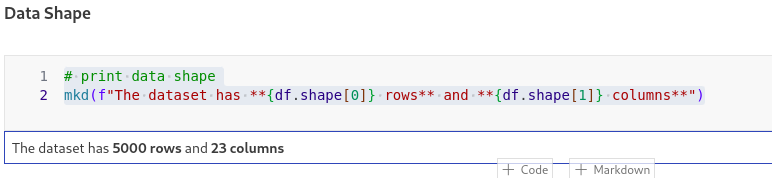
\includegraphics[width=\textwidth]{data_shape.png}
	\caption{Dataset shape \label{fig:data_shape}}
\end{figure} 

\begin{figure}[H]
	% h for here
	% center the image 
	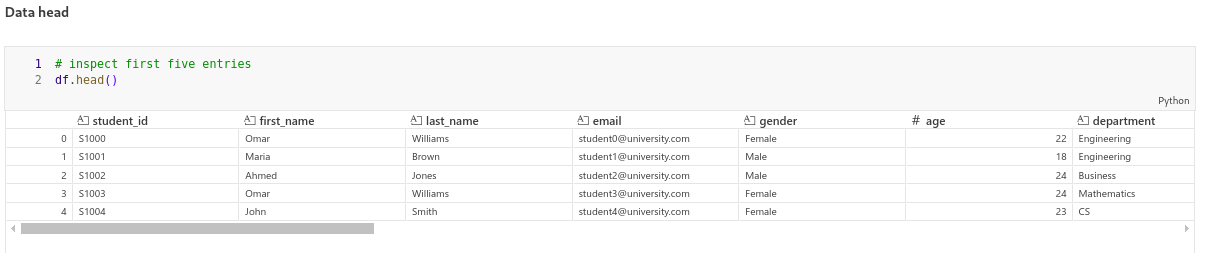
\includegraphics[width=\textwidth]{data_head.png}
	\caption{Dataset Head \label{fig:data_head}}
\end{figure}

\begin{figure}[H]
	% h for here
	% center the image 
	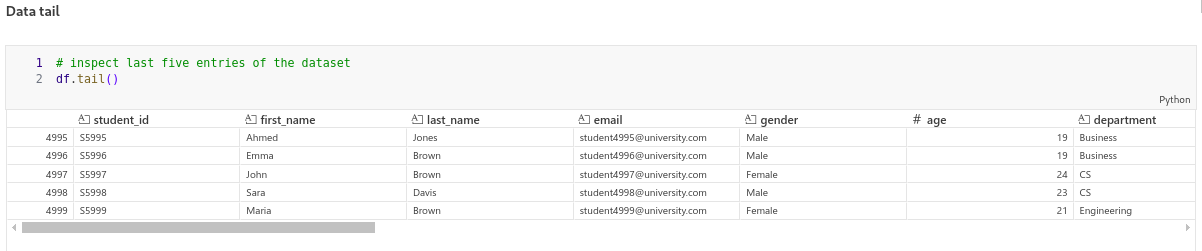
\includegraphics[width=\textwidth]{data_tail.png}
	\caption{Dataset Tail \label{fig:data_tail}}
\end{figure}




\begin{figure}[H] % h for here
	\centering % center the image 
	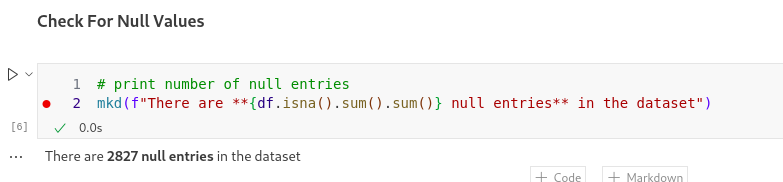
\includegraphics[width=\textwidth]{total_null_values.png}
	\caption{Total number of null values \label{fig:total_null_values}}
\end{figure}

\begin{figure} % h for here
	\centering % center the image 
	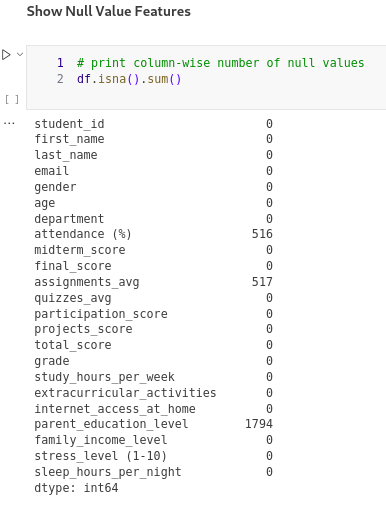
\includegraphics[width=\textwidth]{null_values_dist.png}
	\caption{Null values distribution by features \label{fig:null_values_dist}}
\end{figure}

\begin{figure}[H]
	% h for here
	\centering % center the image 
	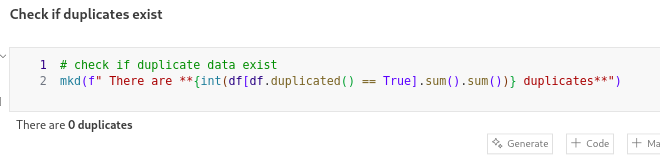
\includegraphics[width=\textwidth]{duplicate_values.png}
	\caption{The number of duplicate values \label{fig:duplicate_values}}
\end{figure}

\begin{figure}[H]
	\centering % center the image 
	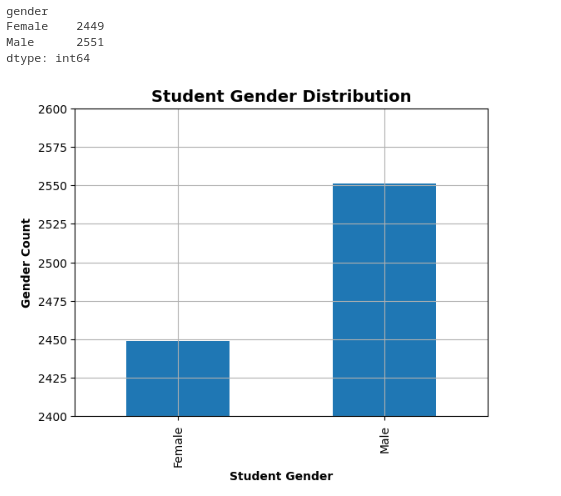
\includegraphics[width=\textwidth]{gender_dist.png}
	\caption{Inconsistent Grades \label{fig:gender_dist}}
\end{figure}

\begin{figure}[H]
	\centering % center the image 
	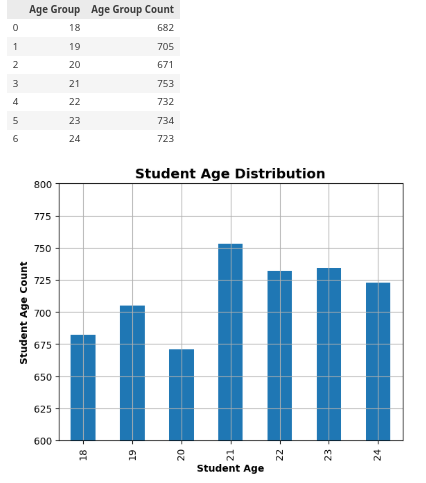
\includegraphics[width=\textwidth]{student_age_dist.png}
	\caption{Student Age Distribution \label{fig:stud_age_dist}}
\end{figure}

\begin{figure}[H]
	\centering % center the image 
	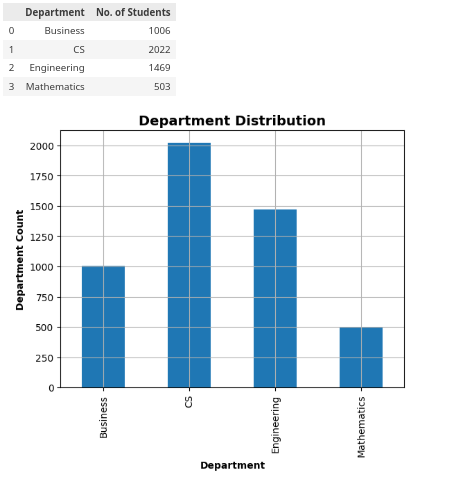
\includegraphics[width=\textwidth]{department_dist.png}
	\caption{Student Department Distribution \label{fig:dept_dist}}
\end{figure}

\begin{figure}[H]
	\centering % center the image 
	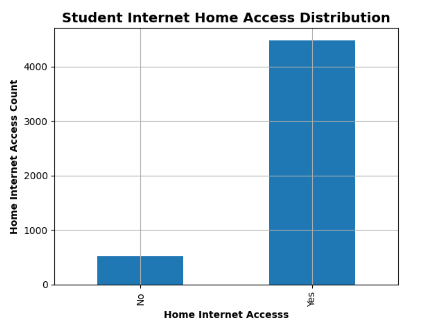
\includegraphics[width=\textwidth]{stud_home_internet.png}
	\caption{Student Home Internet Access Distribution \label{fig:stud_home_internet}}
\end{figure}
\begin{figure}[H]
	\centering % center the image 
	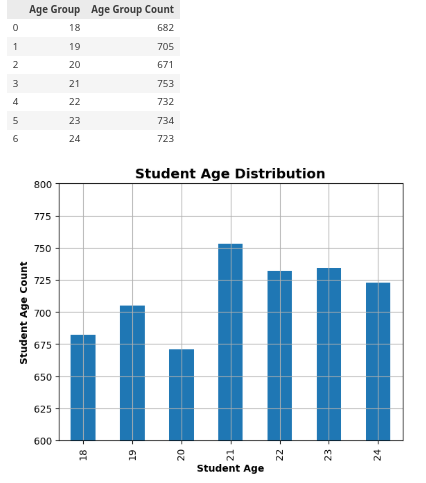
\includegraphics[width=\textwidth]{student_age_dist.png}
	\caption{Student Age Distribution \label{fig:stud_age_dist}}
\end{figure}
\begin{figure}[H]
	\centering % center the image 
	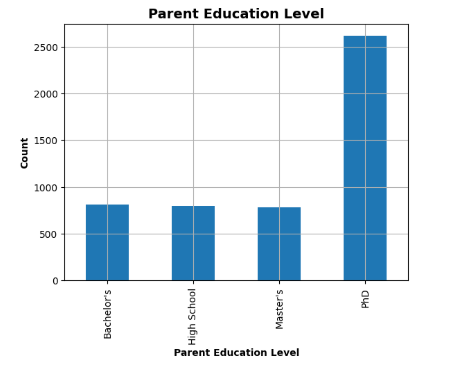
\includegraphics[width=\textwidth]{parent_edu.png}
	\caption{Student Parent Education Level Distribution \label{fig:parent_edu}}
\end{figure}


\begin{figure}[H]
	\centering % center the image 
	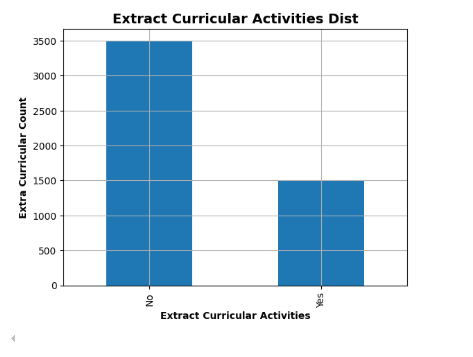
\includegraphics[width=\textwidth]{extra_curricular.png}
	\caption{Student Extra Curricular Distribution \label{fig:extra_curricular}}
\end{figure}

\begin{figure}[H]
	\centering % center the image 
	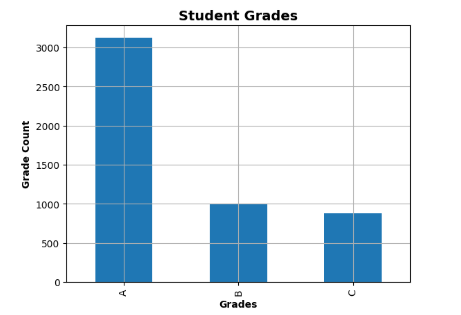
\includegraphics[width=\textwidth]{stud_grade.png}
	\caption{Student Extra Curricular Distribution \label{fig:stud_grade}}
\end{figure}


\begin{figure}[H]
	\centering % center the image 
	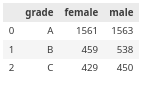
\includegraphics[width=\textwidth]{gender_grade_nums.png}
	\caption{Student Extra Curricular Distribution \label{fig:gender_grade_nums}}
\end{figure}


\begin{figure}[H]
	\centering % center the image 
	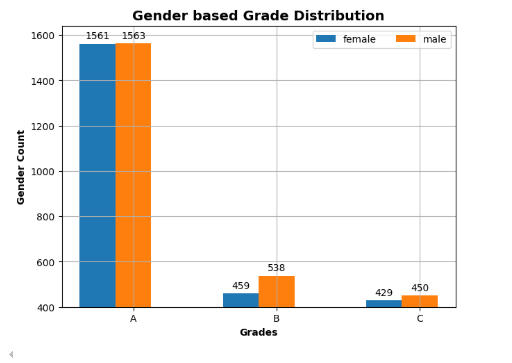
\includegraphics[width=\textwidth]{gender_grade_fig.png}
	\caption{Student Extra Curricular Distribution \label{fig:gender_grade_fig}}
\end{figure}




\begin{figure}[H]
	\centering % center the image 
	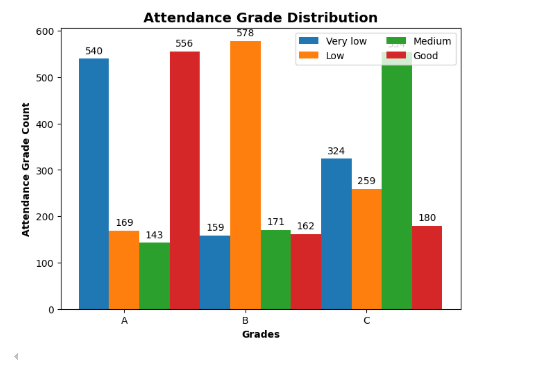
\includegraphics[width=\textwidth]{attendance_grade.png}
	\caption{Student Extra Curricular Distribution \label{fig:attendance_grade}}
\end{figure}

\begin{figure}[H]
	\centering % center the image 
	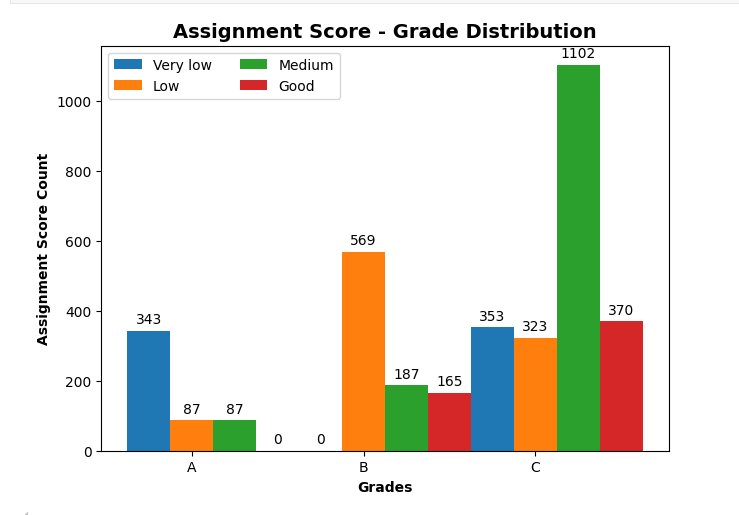
\includegraphics[width=\textwidth]{assignment_score_grade_dist.png}
	\caption{Student Assignment Score Distribution \label{fig:assignment_score_grade_dist}}
\end{figure}



	
\begin{figure}[H]
	\centering 
	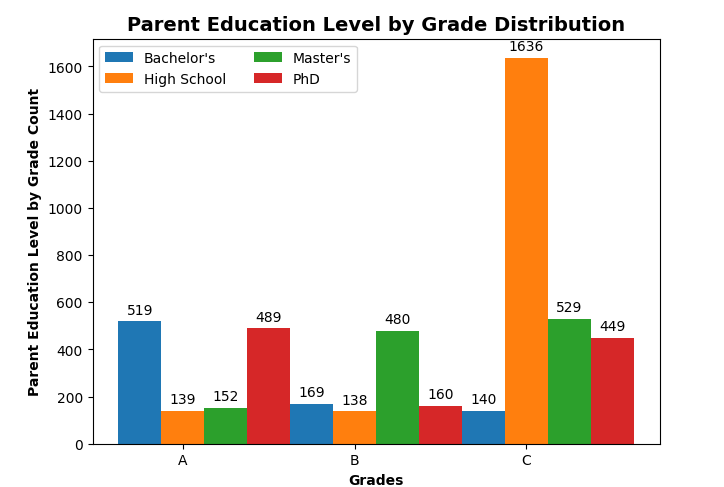
\includegraphics[width=\textwidth]{parent_edu_grade.png}
	\caption{Student parent educational level and grade distribution. \label{fig:parent_edu_level}}
\end{figure}

\begin{figure}[H]
	\centering 
	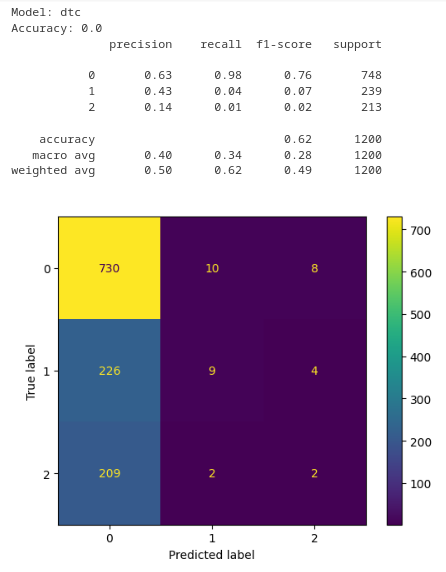
\includegraphics[width=\textwidth]{best_model.png}
	\caption{Best performing model.  \label{fig:best_model}}
\end{figure}

	%\addcontentsline{toc}{chapter}{Visualizations}
	
	
	\appendix
	\chapter*{Appendix}
	\addcontentsline{toc}{chapter}{Appendix}
	
\captionof{listing}{Import Needed Python Packages}
\label{code:import_packages}
\begin{minted}{python}
# import libraries
import numpy as np
import pandas as pd
import matplotlib.pyplot as plt
import seaborn as sns 
from IPython.display import Markdown as mkd 

from sklearn.preprocessing import LabelEncoder
from sklearn.preprocessing import StandardScaler
from sklearn.model_selection import train_test_split
from sklearn.metrics import mean_absolute_error, root_mean_squared_error, mean_absolute_error


from collections import Counter
\end{minted}

\captionof{listing}{Functions Used}
\label{code:functions_used}
\begin{minted}{python}
# Functions used
# These are the functions used in the task

# function to fix grading inconsistent issue.
"""
Using; https://www.mastersportal.com/articles/2290/how-to-convert-uk-grades-for-masters-degrees-in-other-countries.html

Converting British grades into American grades
In the US, the grading system uses letters A-F (without E) to evaluate students. D is the minimum passing grade.

+70% = A
60-69% = B
50-59% = C
40-49% = D
Below 40% = F (fail)
"""
def grader(total_score):
"""
This function is used to compute grades for the students. 
This also applies a known, global and generally accepted grading system.
The input is the total score.
"""
"""Grades : A, B, C, D, E, F"""
if isinstance(total_score, int) or isinstance(total_score, float):
if total_score < 40:
return 'F'
# elif total_score <= 50:
#     return 'E' 
elif total_score <= 49:
return 'D' 
elif total_score <= 59:
return 'C'
elif total_score <= 69:
return 'B' 
else:
return 'A'
else:
raise "Wrong value type. Int or float required" 
\end{minted}


\captionof{listing}{Load dataset in}
\label{code:load_dataset}
\begin{minted}{python}
# load the dataset in the stud_record variable
stud_record = pd.read_csv("datasets/Students_Grading_Dataset.csv")

# convert all features to lovercase 
stud_record.columns = [col.lower() for col in stud_record.columns]
\end{minted}

\captionof{listing}{Show data shape}
\label{code:data_shape}
\begin{minted}{python}
# print data shape
mkd(f"The dataset has **{stud_record.shape[0]} rows** and **{stud_record.shape[1]} columns**")
\end{minted}

\captionof{listing}{Show data head}
\label{code:data_head}
\begin{minted}{python}
# inspect first five entries 
stud_record.head()
\end{minted}

\captionof{listing}{Show dataset head}
\label{code:dataset_head}
\begin{minted}{python}
# inspect first five entries 
stud_record.head()
\end{minted}


\captionof{listing}{Show dataset tail}
\label{code:dataset_tail}
\begin{minted}{python}
# inspect first five entr# inspect last five entries of the dataset
stud_record.tail()
\captionof{listing}{Show inconsistent grading}
\label{code:inconsistent_grading}
\begin{minted}{python}
stud_record[['total_score', 'final_score', 'grade']]
\end{minted}

\captionof{listing}{Show dataset total null values}
\label{code:total_null_values}
\begin{minted}{python}
# inspect first five entr
# print number of null entries
mkd(f"There are **{stud_record.isna().sum().sum()} null entries** in the dataset")
\end{minted}


\captionof{listing}{Show data nulls}
\label{code:dataset_null}
\begin{minted}{python}
# inspect first five entr
# print column-wise number of null values
stud_record.isna().sum()
\end{minted}

\captionof{listing}{Fill null values}
\label{code:fill_null}
\begin{minted}{python}
# let no Assignment_avg mean the student scored 0 in the assignment
# let no Attendance (%) be filled with the most common value, mode as this is not affected by outlier
# let Parent_Education_Level  be filled the mode of the feature as this is not affected by outlier
stud_record.fillna({
	'assignments_avg': 0, 
	'attendance (%)' : stud_record['attendance (%)'].mode()[0],
	'parent_education_level': stud_record['parent_education_level'].mode()[0]},
inplace=True)

# confirm null values filled
stud_record.isna().sum()
\end{minted}


\captionof{listing}{Check for duplicates}
\label{code:duplicates}
\begin{minted}{python}
# check if duplicate data exist
mkd(f" There are **{int(stud_record[stud_record.duplicated() == True].sum().sum())} duplicates**")
\end{minted}


\captionof{listing}{Show descriptive statistics}
\label{code:dataset_head}
\begin{minted}{python}
# Descriptive statistics of the dataset. This can be used to identify outliers
stud_record.describe()
\end{minted}

\captionof{listing}{Confirm datatypes match expected types}
\label{code:dataset_head}
\begin{minted}{python}
# check and confirm each datatype fits the feature name
stud_record.info()
\end{minted}


\captionof{listing}{Show inconsistent grading}
\label{code:inconsistent_grading}
\begin{minted}{python}
stud_record[['total_score', 'final_score', 'grade']]
\end{minted}


\captionof{listing}{Fix inconsistent data type}
\label{code:dataset_head}
\begin{minted}{python}
	stud_record['grade_corrected'] = stud_record['total_score'].apply(grader)
	# show grading inconsistency once more, 
	# investigate accurate fix
	stud_record[['final_score', 'total_score', 'grade', 'grade_corrected']].head()
\end{minted}


\captionof{listing}{Show studetn gender distribution}
\label{code:dataset_head}
\begin{minted}{python}
	# students gender distribution
	gender_distr = stud_record.groupby(by='gender').size()
	
	gender_distr.plot(kind='bar')
	plt.title('Student Gender Distribution', fontdict={'size':14, 'fontweight':'bold'})
	plt.xlabel('Student Gender', fontdict={'fontweight':'bold'})
	plt.ylabel('Gender Count', fontdict={'fontweight':'bold'})
	plt.ylim(2400, 2600)
	plt.grid()
	
	# show gender distribution figures
	gender_distr
\end{minted}


\captionof{listing}{Show student age distribution}
\label{code:student_age}
\begin{minted}{python}
	# student age distribution
	age_dist = stud_record.groupby(by = 'age').size()
	age_dist.plot(kind='bar')
	plt.ylim(600, 800)
	plt.grid()
	plt.title("Student Age Distribution", fontdict={'size':14, 'fontweight':'bold'})
	plt.xlabel('Student Age', fontdict={'fontweight':'bold'})
	plt.ylabel("Student Age Count", fontdict={'fontweight':'bold'})
	
	
	# pd.DataFrame([age_dist.values, age_dist.index], columns=['Numbers', 'values'])
	age_dist.index
	pd.DataFrame({'Age Group': age_dist.index, 'Age Group Count': age_dist.values})
	
\end{minted}


\captionof{listing}{Student department distribution}
\label{code:student_department}
\begin{minted}{python}
	
	# group dataset by department and get size of each department
	dept_dist = stud_record.groupby(by='department').size()
	dept_dist.plot(kind='bar')
	plt.title('Department Distribution', fontdict={'size':14, 'fontweight':'bold'})
	plt.xlabel('Department', fontdict={'fontweight':'bold'})
	plt.ylabel('Department Count', fontdict={'fontweight':'bold'})
	plt.grid()
	# plt.show()
	
	pd.DataFrame({'Department':dept_dist.index, "No. of Students": dept_dist.values})
\end{minted}


\captionof{listing}{Show attendance plot}
\label{code:dataset_head}
\begin{minted}{python}
	# plot student attendance
	stud_record['attendance (%)'].plot()
	plt.title("Attendance Plot [First 100]", fontdict={'size':14, 'fontweight':'bold'})
	plt.xlabel("Student Attendance", fontdict={'fontweight':'bold'})
	plt.ylabel("Student Attendance (%)", fontdict={'fontweight':'bold'})
	plt.xlim(1, 100)
	plt.show()
\end{minted}


\captionof{listing}{Show midterm score}
\label{code:midterm_score}
\begin{minted}{python}
	
	# midterm_score plot of first 100 students
	stud_record['midterm_score'].plot()
	plt.xlim(1,100)
	plt.title("Midterm Score plot [First 100]", fontdict={'size':14, 'fontweight':'bold'})
	plt.xlabel("Midterm score", fontdict={'fontweight':'bold'})
	plt.ylabel("Midterm score count", fontdict={'fontweight':'bold'})
	plt.show()
\end{minted}

\captionof{listing}{Final score plot for the first 200 students}
\label{code:final_score}
\begin{minted}{python}
# Final Score Plot
stud_record['final_score'].plot()
plt.xlim(1,100)
plt.title("Final Score [First 200]", fontdict={'size':14, 'fontweight':'bold'})
plt.xlabel("Final Score", fontdict={'fontweight':'bold'})
plt.ylabel('Final Score Count', fontdict={'fontweight':'bold'})

plt.show()
\end{minted}

% end of univariate analysis
\captionof{listing}{Student Internet Home Access Distribution}
\label{code:internet_access}
\begin{minted}{python}
# dataset grouping by internet_access_at_home and getting the sizes
internet_access_at_home = stud_record.groupby(by='internet_access_at_home').size()

internet_access_at_home.plot(kind='bar')
plt.title('Student Internet Home Access Distribution', fontdict={'size':14, 'fontweight':'bold'})
plt.xlabel('Home Internet Accesss', fontdict={'fontweight':'bold'})
plt.ylabel('Home Internet Access Count', fontdict={'fontweight':'bold'})
# plt.ylim(2400, 2600)
plt.grid()
\end{minted}


\captionof{listing}{Student family income level distribution}
\label{code:family_income}
\begin{minted}{python}
Counter(stud_record.family_income_level)

family_income_level = stud_record.groupby(by='family_income_level').size()

family_income_level.plot(kind='bar')
plt.title('Student Family Income Level Distribution', fontdict={'size':14, 'fontweight':'bold'})
plt.xlabel('Student Family Income Level', fontdict={'fontweight':'bold'})
plt.ylabel('Student Family Income Level Count', fontdict={'fontweight':'bold'})
plt.ylim(1000)
plt.grid()
\end{minted}



\captionof{listing}{Student stress level}
\label{code:stress_level}
\begin{minted}{python}
	
# group dataset by stress_level(1-10) and get size of each stress level
stress_level = stud_record.groupby(by='stress_level (1-10)').size()
stress_level = pd.DataFrame(stress_level) 
stress_level.plot(kind='bar')
plt.title('Student Stress Level Distribution', fontdict={'size':14, 'fontweight':'bold'})
plt.xlabel('Student Stress Level', fontdict={'fontweight':'bold'})
plt.ylabel('Student Stress Level Count', fontdict={'fontweight':'bold'})
plt.ylim(400)
plt.grid()
plt.show();
\end{minted}


\captionof{listing}{Student parent educational level}
\label{code:parent_education}
\begin{minted}{python}
# dataset grouped by paretn_education_level and the different sizes obtained
parent_education = stud_record.groupby(by='parent_education_level').size()
parent_education.plot(kind='bar')
plt.title("Parent Education Level", fontdict={'fontweight':'bold', 'fontsize':14})
plt.xlabel('Parent Education Level', fontdict = {'fontweight':'bold', 'fontsize':10})
plt.ylabel('Count', fontdict={'fontweight':'bold', 'fontsize':10})
plt.grid()

plt.show();
\end{minted}


\captionof{listing}{Student extra curricular activities}
\label{code:extra_curricular}
\begin{minted}{python}
# data grouped by extra curricular activities of student. Size of yes / no extracted
extracurricular = stud_record.groupby(by='extracurricular_activities').size()

extracurricular.plot(kind='bar')
plt.title('Extrac Curricular Activities Dist', fontdict={'fontweight':'bold', 'size':14})
plt.xlabel('Extrac Curricular Activities', fontdict={'fontweight':'bold', 'size':10})
plt.ylabel('Extra Curricular Count', fontdict={'fontweight':'bold', 'size':10})
plt.grid()
plt.show()
\end{minted}


\captionof{listing}{Student grade distribution}
\label{code:grade_dist}
\begin{minted}{python}
	
# group dataset by grade_corrected and get size of each grade
grade = stud_record.groupby(by='grade_corrected').size()
grade.plot(kind='bar')
plt.title("Student Grades", fontdict={'fontweight':'bold', 'size':14})
plt.xlabel('Grades', fontdict={'fontweight':'bold', 'size':10})
plt.ylabel('Grade Count', fontdict={'fontweight':'bold', 'size':10})
plt.grid()

plt.show()
\end{minted}


\captionof{listing}{Gender grade distribution}
\label{code:gender_grade}
\begin{minted}{python}

# group dataset by grade_corrected and gender
gender_grade = stud_record.groupby(by=['grade_corrected', 'gender']).count()['student_id'].reset_index()
gender_grade

valuez = np.array(gender_grade['student_id'])
rows = gender_grade['grade_corrected'].unique() # rows to be plotted
num_rows = int(len(gender_grade['grade_corrected'].unique())) # num of rows for reshaping
num_cols = int(len(gender_grade) / len(rows))   # num of cols for reshaping

data = pd.DataFrame(valuez.reshape((num_rows, num_cols)),
index=pd.Index(list(rows), name='grade'),
columns=pd.Index(['female','male'], name=''))
data = data.reset_index()
data
\end{minted}


\captionof{listing}{Grade by department distribution}
\label{code:grade_department}
\begin{minted}{python}

# investigation of grade-department relationship
department_grade = stud_record.groupby(by = ['grade_corrected', 'department']).size().reset_index()
department_grade

rows = department_grade['grade_corrected'].unique() # rows to be plotted
num_rows = int(len(department_grade['grade_corrected'].unique())) # num of rows for reshaping
num_cols = int(len(department_grade) / len(rows))   # num of cols for reshaping

data = pd.DataFrame(department_grade[0].values.reshape(num_rows, num_cols), 
index=pd.Index(list(rows), name='grade'),
columns = department_grade['department'].unique()
)
data = data.reset_index()

grades = tuple(data['grade'].values)
scores = {
	data.columns[1] : tuple(data[data.columns[1]].values),
	data.columns[2] : tuple(data[data.columns[2]].values),
	data.columns[3] : tuple(data[data.columns[3]].values),
	data.columns[4] : tuple(data[data.columns[4]].values),
}

x = np.arange(len(grades))
width = 0.25 # bar width
multiplier = 0

fig, ax = plt.subplots(layout='constrained')

for attribute, measurement in scores.items():
offset = width * multiplier 
rects = ax.bar(x + offset, measurement, width, label = attribute)
ax.bar_label(rects, padding=3)
multiplier += 1

# Add some text for labels, title and custom x-axis tick labels etc
ax.set_ylabel("ylable")
ax.set_title("Title here", fontdict={'fontweight':'bold', 'size':14})
ax.set_xticks(x + width, rows)
ax.legend(loc='upper right', ncols = len(rows) - 1)
# ax.set_ylim()
plt.xlabel('Grades', fontdict={'fontweight':'bold', 'size':10})
plt.ylabel('Department Grade Distrution', fontdict={'fontweight':'bold', 'size':10})
plt.title('Department Grade Distribution', fontdict={'fontweight':'bold', 'size':14})

plt.show()
\end{minted}



\captionof{listing}{Grade by attendance distribution}
\label{code:grade_attendance}
\begin{minted}{python}
	
# making a deep copy of the dataframe 
stud_record_updated = stud_record.copy()

# Confirm the two records are different
stud_record_updated is stud_record

labels = ["Very low", "Low", "Medium", "Good", 'Very good']

stud_record_updated['attendance_classified'] = pd.cut(np.array(list(stud_record_updated['attendance (%)'])), len(labels), labels = labels)
attendance_grade = stud_record_updated.groupby(by = ['attendance_classified', 'grade_corrected'], observed=False).size().reset_index()

rows = attendance_grade['grade_corrected'].unique()
num_rows = int(len(attendance_grade['grade_corrected'].unique())) # num of rows for reshaping
num_cols = int(len(attendance_grade) / len(rows))   # num of cols for reshaping

data = pd.DataFrame(attendance_grade[0].values.reshape(num_rows, num_cols), 
index=pd.Index(list(rows), name='grade'),
columns = attendance_grade['attendance_classified'].unique()
)
data = data.reset_index()
grades = tuple(data['grade'].values)
scores = {
	data.columns[1] : tuple(data[data.columns[1]].values),
	data.columns[2] : tuple(data[data.columns[2]].values),
	data.columns[3] : tuple(data[data.columns[3]].values),
	data.columns[4] : tuple(data[data.columns[4]].values),
}

x = np.arange(len(grades))
width = 0.25 # bar width
multiplier = 0

fig, ax = plt.subplots(layout='constrained')

for attribute, measurement in scores.items():
offset = width * multiplier 
rects = ax.bar(x + offset, measurement, width, label = attribute)
ax.bar_label(rects, padding=3)
multiplier += 1

# Add some text for labels, title and custom x-axis tick labels etc
ax.set_ylabel("ylable")
ax.set_title("Title here", fontdict={'fontweight':'bold', 'size':14})
ax.set_xticks(x + width, rows)
ax.legend(loc='upper right', ncols = len(rows) - 1)
# ax.set_ylim()
plt.xlabel('Grades', fontdict={'fontweight':'bold', 'size':10})
plt.ylabel('Attendance Grade Count', fontdict={'fontweight':'bold', 'size':10})
plt.title('Attendance Grade Distribution', fontdict={'fontweight':'bold', 'size':14})

plt.show();
\end{minted}


\captionof{listing}{Grade by assignment distribution}
\label{code:grade_assignment}
\begin{minted}{python}
	
# Assignments Avg Score Distribution was classified as Very low, Low, Medium, Good, Very good
stud_record_updated['assignment_classified'] = pd.cut(np.array(list(stud_record_updated['assignments_avg'])), len(labels), labels = labels)
assignment_avg = stud_record_updated.groupby(by = ['assignment_classified', 'grade_corrected'], observed=False).size().reset_index()


# stud_record_updated['assignment_avg_classified'] = pd.cut(np.array(list(stud_record_updated['assignments_avg'])), len(labels), labels = labels)
# assignment_avg = stud_record_updated.groupby(by = ['assignment_avg_classified', 'grade_corrected'], observed=False).size().reset_index()

rows = assignment_avg['grade_corrected'].unique()
num_rows = int(len(assignment_avg['grade_corrected'].unique())) # num of rows for reshaping
num_cols = int(len(assignment_avg) / len(rows))   # num of cols for reshaping

data = pd.DataFrame(assignment_avg[0].values.reshape(num_rows, num_cols), 
index=pd.Index(list(rows), name='grade_corrected'),
columns = assignment_avg['assignment_classified'].unique()
)

data = data.reset_index()
grades = tuple(data['grade_corrected'].values)
scores = {
	data.columns[1] : tuple(data[data.columns[1]].values),
	data.columns[2] : tuple(data[data.columns[2]].values),
	data.columns[3] : tuple(data[data.columns[3]].values),
	data.columns[4] : tuple(data[data.columns[4]].values),
}

x = np.arange(len(grades))
width = 0.25 # bar width
multiplier = 0

fig, ax = plt.subplots(layout='constrained')

for attribute, measurement in scores.items():
offset = width * multiplier 
rects = ax.bar(x + offset, measurement, width, label = attribute)
ax.bar_label(rects, padding=3)
multiplier += 1

# Add some text for labels, title and custom x-axis tick labels etc
ax.set_ylabel("ylable")
ax.set_title("Title here", fontdict={'fontweight':'bold', 'size':14})
ax.set_xticks(x + width, rows)
ax.legend(loc='upper left', ncols = len(rows) - 1)
# ax.set_ylim()
plt.xlabel('Grades', fontdict={'fontweight':'bold', 'size':10})
plt.ylabel('Assignment Score Count', fontdict={'fontweight':'bold', 'size':10})
plt.title('Assignment Score - Grade Distribution', fontdict={'fontweight':'bold', 'size':14})

plt.show();
\end{minted}



\captionof{listing}{Grade by quizz score distribution}
\label{code:grade_quizz_score}
\begin{minted}{python}
	
stud_record_updated['quizzes_avg_classified'] = pd.cut(np.array(list(stud_record_updated['quizzes_avg'])), len(labels), labels = labels)
assignment_avg = stud_record_updated.groupby(by = ['assignment_classified', 'grade_corrected'], observed=False).size().reset_index()


# stud_record_updated['assignment_avg_classified'] = pd.cut(np.array(list(stud_record_updated['assignments_avg'])), len(labels), labels = labels)
# assignment_avg = stud_record_updated.groupby(by = ['assignment_avg_classified', 'grade_corrected'], observed=False).size().reset_index()

rows = assignment_avg['grade_corrected'].unique()
num_rows = int(len(assignment_avg['grade_corrected'].unique())) # num of rows for reshaping
num_cols = int(len(assignment_avg) / len(rows))   # num of cols for reshaping
num_cols

data = pd.DataFrame(assignment_avg[0].values.reshape(num_rows, num_cols), 
index=pd.Index(list(rows), name='grade_corrected'),
columns = assignment_avg['assignment_classified'].unique()
)

data = data.reset_index()
grades = tuple(data['grade_corrected'].values)
scores = {
	data.columns[1] : tuple(data[data.columns[1]].values),
	data.columns[2] : tuple(data[data.columns[2]].values),
	data.columns[3] : tuple(data[data.columns[3]].values),
	data.columns[4] : tuple(data[data.columns[4]].values),
}

x = np.arange(len(grades))
width = 0.25 # bar width
multiplier = 0

fig, ax = plt.subplots(layout='constrained')

for attribute, measurement in scores.items():
offset = width * multiplier 
rects = ax.bar(x + offset, measurement, width, label = attribute)
ax.bar_label(rects, padding=3)
multiplier += 1

# Add some text for labels, title and custom x-axis tick labels etc
ax.set_ylabel("ylable")
ax.set_title("Title here", fontdict={'fontweight':'bold', 'size':14})
ax.set_xticks(x + width, rows)
ax.legend(loc='upper left', ncols = len(rows) - 1)
# ax.set_ylim()
plt.xlabel('Grades', fontdict={'fontweight':'bold', 'size':10})
plt.ylabel('Quizz Score Count', fontdict={'fontweight':'bold', 'size':10})
plt.title('Quizz Score Distribution', fontdict={'fontweight':'bold', 'size':14})

plt.show();
	
\end{minted}



\captionof{listing}{Grade by study hours per week distribution}
\label{code:grade_department}
\begin{minted}{python}
	
stud_record_updated['study_hours_per_week_classified'] = pd.cut(np.array(list(stud_record_updated['study_hours_per_week'])), len(labels), labels = labels)
assignment_avg = stud_record_updated.groupby(by = ['study_hours_per_week_classified', 'grade_corrected'], observed=False).size().reset_index()

rows = assignment_avg['grade_corrected'].unique()
num_rows = int(len(assignment_avg['grade_corrected'].unique())) # num of rows for reshaping
num_cols = int(len(assignment_avg) / len(rows))   # num of cols for reshaping
num_cols

data = pd.DataFrame(assignment_avg[0].values.reshape(num_rows, num_cols), 
index=pd.Index(list(rows), name='grade_corrected'),
columns = assignment_avg['study_hours_per_week_classified'].unique()
)

data = data.reset_index()
grades = tuple(data['grade_corrected'].values)
scores = {
	data.columns[1] : tuple(data[data.columns[1]].values),
	data.columns[2] : tuple(data[data.columns[2]].values),
	data.columns[3] : tuple(data[data.columns[3]].values),
	data.columns[4] : tuple(data[data.columns[4]].values),
}

x = np.arange(len(grades))
width = 0.25 # bar width
multiplier = 0

fig, ax = plt.subplots(layout='constrained')

for attribute, measurement in scores.items():
offset = width * multiplier 
rects = ax.bar(x + offset, measurement, width, label = attribute)
ax.bar_label(rects, padding=3)
multiplier += 1

# Add some text for labels, title and custom x-axis tick labels etc
ax.set_ylabel("ylable")
ax.set_title("Title here", fontdict={'fontweight':'bold', 'size':14})
ax.set_xticks(x + width, rows)
ax.legend(loc='upper left', ncols = len(rows) - 1)
# ax.set_ylim()
plt.xlabel('Grades', fontdict={'fontweight':'bold', 'size':10})
plt.ylabel('Quizz Score Count', fontdict={'fontweight':'bold', 'size':10})
plt.title('Quizz Score Distribution', fontdict={'fontweight':'bold', 'size':14})

plt.show();
	
\end{minted}


\captionof{listing}{Label encoding and scaling functions}
\label{code:encoding_scaling}
\begin{minted}{python}
def encoder(dataframe, val = LabelEncoder):
""" 
Function accepts dataframe and uses the encoding method passed in to encode the categorical data
argument: dataframe to be encoded
returns encoded dataframe
"""
le = val()

for feature in dataframe:
dataframe[feature] = le.fit_transform(dataframe[feature])

return dataframe 

def scaler(dataframe):
"""
Function normalizes data before it is used in machine learning model. This process makes it easier for models to understand
the features and predict them better.
argument is the dataframe to be scaled.
return : scaled dataframe 
"""
standard_scaler = StandardScaler()
return standard_scaler.fit_transform(dataframe)

# # inspect result
# stud_encoded = encoder(stud_record_choice_features).head()
# scaler(stud_encoded)
\end{minted}


\captionof{listing}{X and y features separation}
\label{code:x_y}
\begin{minted}{python}
# select dependent and independent features
X_features = stud_record_choice_features.drop('grade_corrected', axis='columns')
y_feature = stud_record_choice_features['grade_corrected']

# split data into train test set
X_features_train, X_features_test, y_feature_train, y_feature_test = train_test_split(X_features, y_feature, train_size=0.7, random_state=42)

# create validation test set
X_features_test, X_features_valid, y_feature_test, y_feature_valid = train_test_split(X_features_test, y_feature_test, train_size=0.8, random_state=42)
\end{minted}

\captionof{listing}{heading}
\label{code:encoding_and_scaling}
\begin{minted}{python}
# encode and scale parameters
X_train = scaler(encoder(X_features_train.select_dtypes(include='object')))
X_test = scaler(encoder(X_features_test.select_dtypes(include='object')))
X_valid = scaler(encoder(X_features_valid.select_dtypes(include='object')))

le = LabelEncoder()
y_train = le.fit_transform(y_feature_train)
y_test = le.fit_transform(y_feature_test) 
y_valid = le.fit_transform(y_feature_valid)
\end{minted}


\captionof{listing}{Import model building packages}
\label{code:modeling_packages}
\begin{minted}{python}
# import modelling packages
from xgboost import XGBClassifier
from sklearn.tree import DecisionTreeClassifier
from sklearn.ensemble import RandomForestClassifier
from sklearn.metrics import classification_report
from sklearn.metrics import confusion_matrix
from sklearn.metrics import accuracy_score
from sklearn.metrics import ConfusionMatrixDisplay
\end{minted}


\captionof{listing}{Model dictionary}
\label{code:model_dict}
\begin{minted}{python}
# building baseline model
models = {
	'xgb' : XGBClassifier,
	'rdf' : RandomForestClassifier,
	'dtc' : DecisionTreeClassifier,
}
\end{minted}


\captionof{listing}{Iterate model dictionary, create, train and evaluate models}
\label{code:create_train_evaluate}
\begin{minted}{python}
for model in models:
print(f"Model: {model}")
clf = models[model]()
clf.fit(X_train, y_feature_train)
y_pred = clf.predict(X_test)
print(f"Accuracy: {accuracy_score(y_feature_test, y_pred)}")
print(classification_report(y_test, y_pred))
cm = confusion_matrix(y_test, y_pred)
disp = ConfusionMatrixDisplay(confusion_matrix=cm, display_labels=clf.classes_)
disp.plot()
plt.show()
\end{minted}
	
	
	%\bibliographystyle{plain}
	\bibliographystyle{agsm}
	\bibliography{bibliography/references.bib}
	\addcontentsline{toc}{chapter}{References}
	
	
	%\input{preliminaries/listoffigures}
	%\addcontentsline{toc}{chapter}{List Of Figures}
	
	%\preto\tabular{\setcounter{magicrownumbers}{0}}
%\newcounter{magicrownumbers}
%\newcommand\rownumber{\stepcounter{magicrownumbers}\arabic{magicrownumbers}}
%\section{List of Tables}

	
%	\begin{tabular}{@{\makebox[1em][r]{\rownumber\space}} | l@{\makebox[1em][r]{}} | l}
%		
%		\multicolumn{0}{@{\makebox[01em]{ID~}} | } | { Features jsdfjsfj sdfj ds df dlfsd fd} | { Featurezz}\\    
%		Something & hello\\
%		Other stuff & hello \\
%		Something something & hello \\
%		MAGIC!  & hello\\ 
%		Something something & hello
%	\end{tabular}
\tableofcontents
	%\addcontentsline{toc}{chapter}{List Of Tables}
		
	
	
\end{document}